\documentclass[a4paper,10pt]{article}

% Hier die Nummer des Blatts und Autoren angeben.
\newcommand{\blatt}{7}
\newcommand{\autor}{Merlin Steuer}

\usepackage{hci}

\begin{document}
% Seitenkopf mit Informationen
\kopf
\renewcommand{\figurename}{Figure}

\aufgabe{11}
Beschrieben werden soll das Produkt londonbeatbox. Es handelt sich um einen kleinen, aber relativ Leistungsstarken Bluetooth-Lautsprecher, welcher Musik vom Handy oder ähnlichen Geräten abspielt. Die Bedienung geschieht komplett über 4 mechanische Elemente - 3 Knöpfe an der Geräteseite (weiter, zurück, play/pause) sowie einem Schieberegler um das Gerät ein- oder auszuschalten. Der Gerätestatus wird über eine LED angezeigt, welche im Gehäuse verbaut ist und u.a. Ladestand und Verbindugnsstatus anzeigen soll.

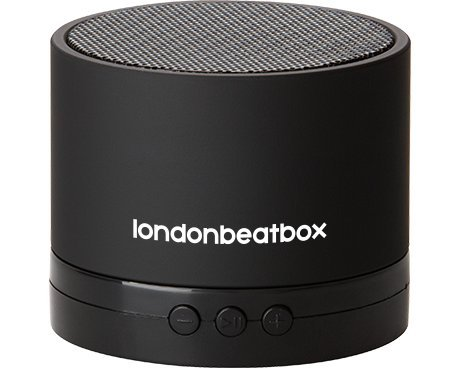
\includegraphics[scale=0.5]{img.jpg}

\subsection{Funktionalität}
\begin{itemize}
    \item Die londonbeatbox tut ihren Job seit einigen Jahren sehr gut. 
    \item Die Funktionalität der seitlichen Tasten ist gegeben
    \item Die eigentliche Steuerung geschieht jedoch i.d.R. über das Mobiltelefon (Start/Stop, Titelwahl etc.)
\end{itemize}

\subsection{Ergonomie}
\begin{itemize}
\item Das Einschalten des Gerätes geht schnell
\item Die Seitlichen Bedienelemente sind jedoch so angebracht, dass bei Benutzung das Gerät oft verrutscht.
\end{itemize}

\subsection{Ästhetik}
\begin{itemize}
\item Das Gerät ist schlicht, schwarz.
\item Es fügt sich unauffällig in die Umgebung ein.
\item Positionierung ist nahezu überall möglich, da unauffälliges Design und
mit Haftstreifen am Boden versehen.
\end{itemize}

\subsection{Erlebnishaftigkeit}
\begin{itemize}
\item Die Grundfunktionalität ist gegeben
\item Das Design ist ansosnten eher schlicht
\item Daher sollte die Bedienung hauptsächlich über das Mobiltelefon statt finden
\item Knöpfe haben unschönen Druckpunkt und Benutzung verschiebt das Gerät.
\end{itemize}

\subsection{Symbolik}
\begin{itemize}
\item Knöpfe sind mit den Üblichen Icons bezeichnet.
\item Status-LED unbrauchbar. Diese ist schlecht zu sehen und die Codierung der einzlenen Blinkfolgen erschließt sich nur mit genauem Blick in die Bedienungsanleitung.
\item Sound-Ausgaben zur Anzeige des Verbindungsstatus aber deutlich und verständlich.
\end{itemize}
\end{document}
